\chapter{The Model Panel}\label{lab:train}

The model panel allows the user to evaluate and train models. The user can switch between both modes using the tab panel below the extraction bar.

\section{Extraction}\label{lab:train_extract_overview}

\begin{figure}[h]
\begin{center}
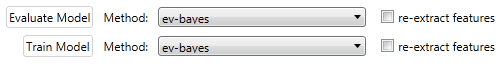
\includegraphics[scale=0.5]{pics/train_gui_extract.png}
\end{center}
\vspace{-0.5cm}
\caption{The extraction bar.}
\label{fig:extract_gui}
\end{figure}

The extraction bar is used by both, the evaluation and the training panel to extract samples using the selected signal and annotation. The extraction methods defines the type of features that will be extracted from the signal and the type of model, which is trained from the extracted samples (see Section \ref{lab:train_extraction}).

To speed up consecutive runs on the same recordings, extracted samples are stored on disk with the following naming convention: \texttt{ <signal>.<annotation>.<method>.samples}. If it becomes necessary to re-extract all samples, e.g.\ because of changed annotations, the check box \texttt{re-extract features} should be checked.

\section{Evaluation}\label{lab:train_eval_overview}

\begin{figure}[h]
\begin{center}
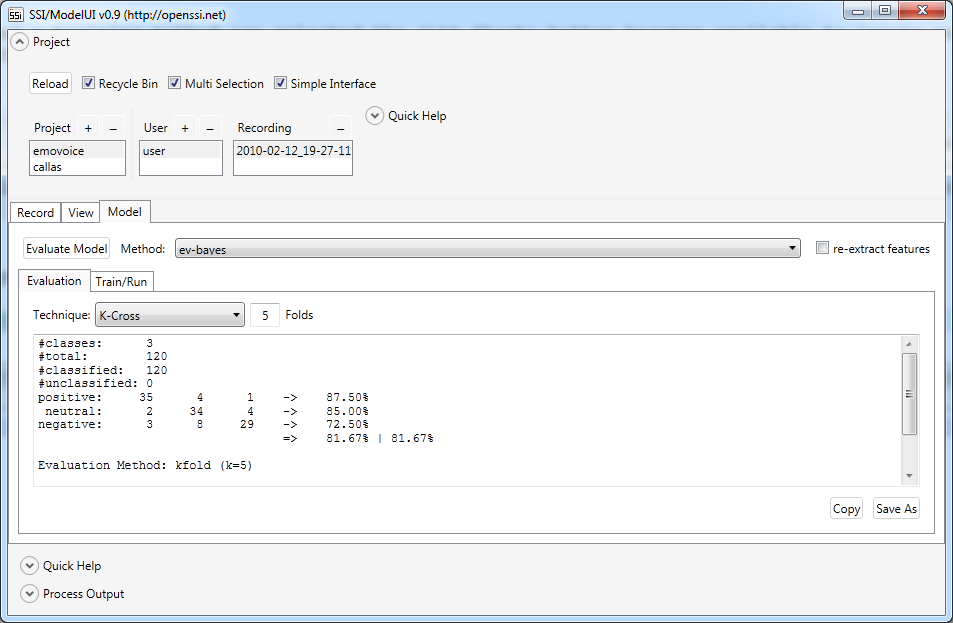
\includegraphics[scale=0.5]{pics/train_gui_eval.png}
\end{center}
\vspace{-0.5cm}
\caption{The evaluation panel.}
\label{fig:eval_gui}
\end{figure}

After selecting at least one recording session and a training method press the \texttt{Start Evaluation} button invoke an evaluation on the selected recording session(s). The following evaluation strategies are available:

\begin{enumerate}
\item{full = the full training corpus will be used for evaluation}
\item{k-fold = the training corpus is split in k folds and each fold is left out once while the others are used to train the model}
\item{leave-one-user-out = one user is completely left out and the others are used for training, which is is repeated for each user}
\item{leave-one-sample-out = one sample is completely left out and the others are used for training, which is is repeated for each sample}
\end{enumerate}

The result of an evaluation is displayed as a confusion matrix and can be copied to the clipboard or stored in a text file.

\section{Training}\label{lab:train_overview}

\begin{figure}[h]
\begin{center}
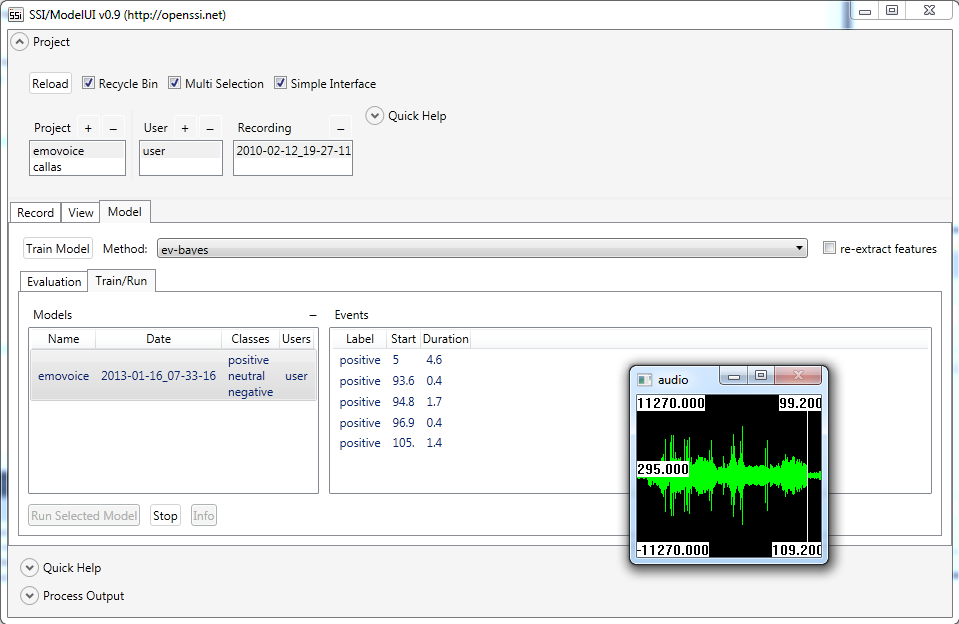
\includegraphics[width=0.75\linewidth]{pics/train_gui_train.png}
\end{center}
\caption{The training panel.}
\label{fig:train_gui}
\end{figure}

When the \texttt{Train/Run} mode is active and the \texttt{Train Model} button is pressed all selected recordings will be used to train a new model. When training is finished the new model is added to the list of available models. For each entry the class names and user names are displayed. Hitting the \texttt{Info} button opens a file with ending \texttt{training}. It is generated during the training procedure and includes relevant information about the training, such as the name of the classifier or the included recordings:
 
\begin{lstlisting}[language=xml]
<training ssi-v="1">
   <def>ev-bayes</def>
   <signal>audio</signal>
   <type>1</type>
   <anno>turns</anno>
   <paths>
      <item>2010-02-12_19-27-11</item>
   </paths>
</training>
\end{lstlisting}
 
Finally, a selected model can be directly tested by pressing \texttt{Run Selected Model}. Detected events are classified in real-time and displayed.

\section{Using a Model}\label{lab:train_overview}

Models can be used outside the GUI in SSI pipelines if you make sure to apply as input the same (possibly pre-processed) signal. Let us pick up the previous example that was using an audio signal and a voice activity detection (VAD) to trigger the recognition component. After putting the audio sensor and a transformer to apply VAD in place, we need two more components to complete the pipeline. A \texttt{ZeroEventSender}, which picks up the VAD signal and sends an event if a non-zero segment of certain length (\texttt{mindur}) is found, and a \texttt{Classifier}, which takes the audio signal and listens to the trigger (here the event address has been set to \texttt{speech@audio}):

\begin{lstlisting}[language=xml]
<consumer create="ssi_consumer_ZeroEventSender" mindur="1.0" hangin="3" hangout="3" sname="audio" ename="speech">
   <input pin="audio_vad" frame="0.1s"/>		  
</consumer>

<consumer create="ssi_consumer_Classifier" trainer="emovoice">
  <input pin="audio" listen="speech@audio">
     <transformer create="ssi_feature_EmoVoiceFeat"/>
  </input>
</consumer>
\end{lstlisting}

Note that it is not necessary to manually apply feature extraction or mention the classification method as these properties are stored along with the trained model, which consists of the following three files:
\begin{itemize}
\item \texttt{emovoice.trainer}
\item \texttt{emovoice.ssi\_model\_NaiveBayes.model}
\item \texttt{emovoice.00.ssi\_feature\_EmoVoiceFeat.option}
\end{itemize}
